\documentclass{standalone}
\usepackage[dvipsnames]{xcolor}
\usepackage{tikz}
\usetikzlibrary{arrows.meta,matrix,positioning,fit}

\colorlet{2bit}{Melon}
\colorlet{4bit}{SkyBlue}
\colorlet{8bit}{LimeGreen}


\begin{document}

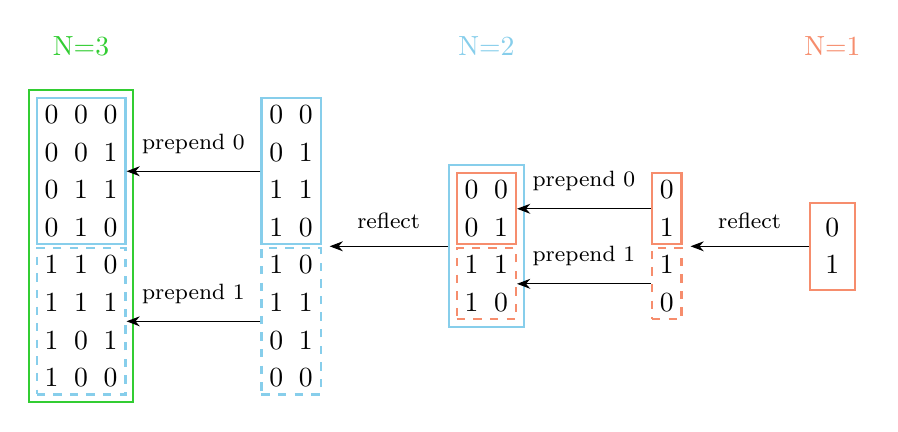
\begin{tikzpicture}[
  outline/.style={thick,inner sep=0mm},
  reversed/.style={dashed},
  graytable/.style={
    outline,
    matrix of nodes,
    nodes={color=black,minimum height=0,outer sep=0},
    column sep=0,
    row sep=0.5mm,
    inner sep=1mm
  }
]
\matrix (G8) [graytable,color=8bit,draw] at (0,1)
{
  0&0&0\\
  0&0&1\\
  0&1&1\\
  0&1&0\\
  1&1&0\\
  1&1&1\\
  1&0&1\\
  1&0&0\\
};

\matrix (G4reflected) [right=1.5cm of G8.east, graytable,color=4bit]
{
  0&0\\
  0&1\\
  1&1\\
  1&0\\
  1&0\\
  1&1\\
  0&1\\
  0&0\\
};

\matrix (G4) [right=1.5cm of G4reflected.east, graytable,color=4bit,draw]
{
  0&0\\
  0&1\\
  1&1\\
  1&0\\
};

\matrix (G2reflected) [right=1.5cm of G4.east, graytable]
{
  0\\
  1\\
  1\\
  0\\
};

\matrix (G2) [right=1.5cm of G2reflected, graytable,draw=2bit]
{
  0\\
  1\\
};

\node[outline,fit={(G2reflected-1-1.north west) (G2reflected-2-1.south east)},draw=2bit] (G2emb){};
\node[outline,reversed,fit={(G2reflected-3-1.north west) (G2reflected-4-1.south east)},draw=2bit] (G2embrev){};

\node[outline,fit={(G4-1-1.north west) (G4-2-2.south east)},draw=2bit] (G2emb2){};
\node[outline,reversed,fit={(G4-3-1.north west) (G4-4-2.south east)},draw=2bit] (G2embrev2){};


\node[outline,fit={(G8-1-1.north west) (G8-4-3.south east)},draw=4bit] (G4emb){};
\node[outline,reversed,fit={(G8-5-1.north west) (G8-8-3.south east)},draw=4bit] (G4embrev){};

\node[outline,fit={(G4reflected-1-1.north west) (G4reflected-4-2.south east)},draw=4bit] (G4emb2){};
\node[outline,reversed,fit={(G4reflected-5-1.north west) (G4reflected-8-2.south east)},draw=4bit] (G4embrev2){};



\draw[-Stealth] (G2) -- node[midway,above=1mm]{\footnotesize reflect} (G2reflected);
\draw[-Stealth] (G2emb) -- node[midway,above=1mm]{\footnotesize prepend 0} (G2emb2);
\draw[-Stealth] (G2embrev) -- node[midway,above=1mm]{\footnotesize prepend 1} (G2embrev2);

\draw[-Stealth] (G4) -- node[midway,above=1mm]{\footnotesize reflect} (G4reflected);

\draw[-Stealth] (G4emb2) -- node[midway,above=1mm]{\footnotesize prepend 0} (G4emb);
\draw[-Stealth] (G4embrev2) -- node[midway,above=1mm]{\footnotesize prepend 1} (G4embrev);


\node [above=3mm of G8,8bit] (N8) {N=3};
\node [4bit] at (N8 -| G4) (N4) {N=2};
\node [2bit] at (N4 -| G2) (N2) {N=1};

\end{tikzpicture}

\end{document}
